\chapter{Mandelbrot Set}

\noindent Mandelbrot Set, është një fraktal i emërtuar pas Benoit B. Mandelbrot, definuar sipas funksionit rekursiv \( z_{n+1} = z_n^2 + c \), ku \( z \) dhe \( c \) janë numra kompleks. Duke filluar me \( z_0 = 0 \), numri kompleks \( c \) i takon Mandelbrot set nëse vargu \( z_n \) është i kufizuar kur \( n \to \infty \). Për shembull, pika \( c = 1 \) nuk është element i bashkësisë Mandelbrot sepse për \( c = 1 \), vargu \( 0, 1, 2, 5, 26 \) tenton në pafundësi. Pika \( c = -1 \) është element i bashkësisë Mandelbrot sepse vargu \( 0, -1, 0, -1, 0, \ldots \) është i kufizuar. Teorema 1 do të na ndihmoj në vizualizimin e fraktalit \cite{complex_analysis}.

\noindent \\ \textbf{Teorema 1.} Numri kompleks \( c \) i takon bashkësisë Mandelbrot atëherë dhe vetëm atëherë kur \( |z_n| \leq 2 \) për çdo \( n \geq 1 \).

\noindent \\Secili piksell i imazhit reprezenton një pikë në sistemin koordinativ dhe për atë pikë e testojme nëse \( |z_n| \leq 2 \) pas \(n_\text{max}\) iterimeve. Nëse me ngjyrë te zezë ngjyrosim pikat që i takojne bashkësisë dhe me ngjyrë të bardhë pikat që nuk i takojnë bashkësisë, atëherë do të fitojmë imazhin në figurën \ref{fig:mandelbrot_bw}.

\begin{figure}[h]
    \centering
    
\includegraphics[width=0.4\linewidth]{mandelbrot_1.png}
    \caption{Mandelbrot Set bardhë dhe e zëzë.}
    \label{fig:mandelbrot_bw}
\end{figure}

\section{Pasqyrimi i piksellëve në sistemin kordinativ}
Për pasqyrim të pikselëve në sistem koordinativ, e përdorim ekuacionin e drejtëzës. Le të jetë 
imazhi \(I\) me dimensione \(w \times h\). Le të jenë pikat \((x_1, y_2)\) dhe \((x_2, y_2)\), pikat e fillimit dhe mbarimit 
të sistemit koordinativ në të cilin imazhi duhet të pasqyrohet si në figurën \ref{fig:image_coordinate}. Secili piksell \((i, j)\) duhet të 
reprezentojë një pikë \((x, y)\) në sistemin koordinativ. Për shembull, pikselli \((0, 0)\) pasqyrohet në \((x_1, y_2)\).


\noindent \\ Intervali $[0,w]$ duhet të pasqyrohet në $[x_1,x_2]$ dhe intervali $[0,h]$ duhet të pasqyrohet në $[y_1,y_2]$. Definojmë pasqyrimet $f_r$, $f_y$ për këto intervale.

\[
f_r : [0, w] \rightarrow [x_1, x_2]
\]
\[
f_c : [0, h] \rightarrow [y_1, y_2]
\]

\noindent \\Për kordinatat \(x\) vlenë
\[
f_r(0) = x_1
\]
\[
f_r(w) = x_2
\]

\noindent Transformimi linear për kordinatat $x$ mund të fitohet si ekuacioni i drejtëzës së pikave $(0, x_1)$ dhe $(w, x_2)$.

\[
\frac{i - 0}{w - 0} = \frac{x - x_1}{x_2 - x_1}
\]

\begin{figure}[h]
    \centering
    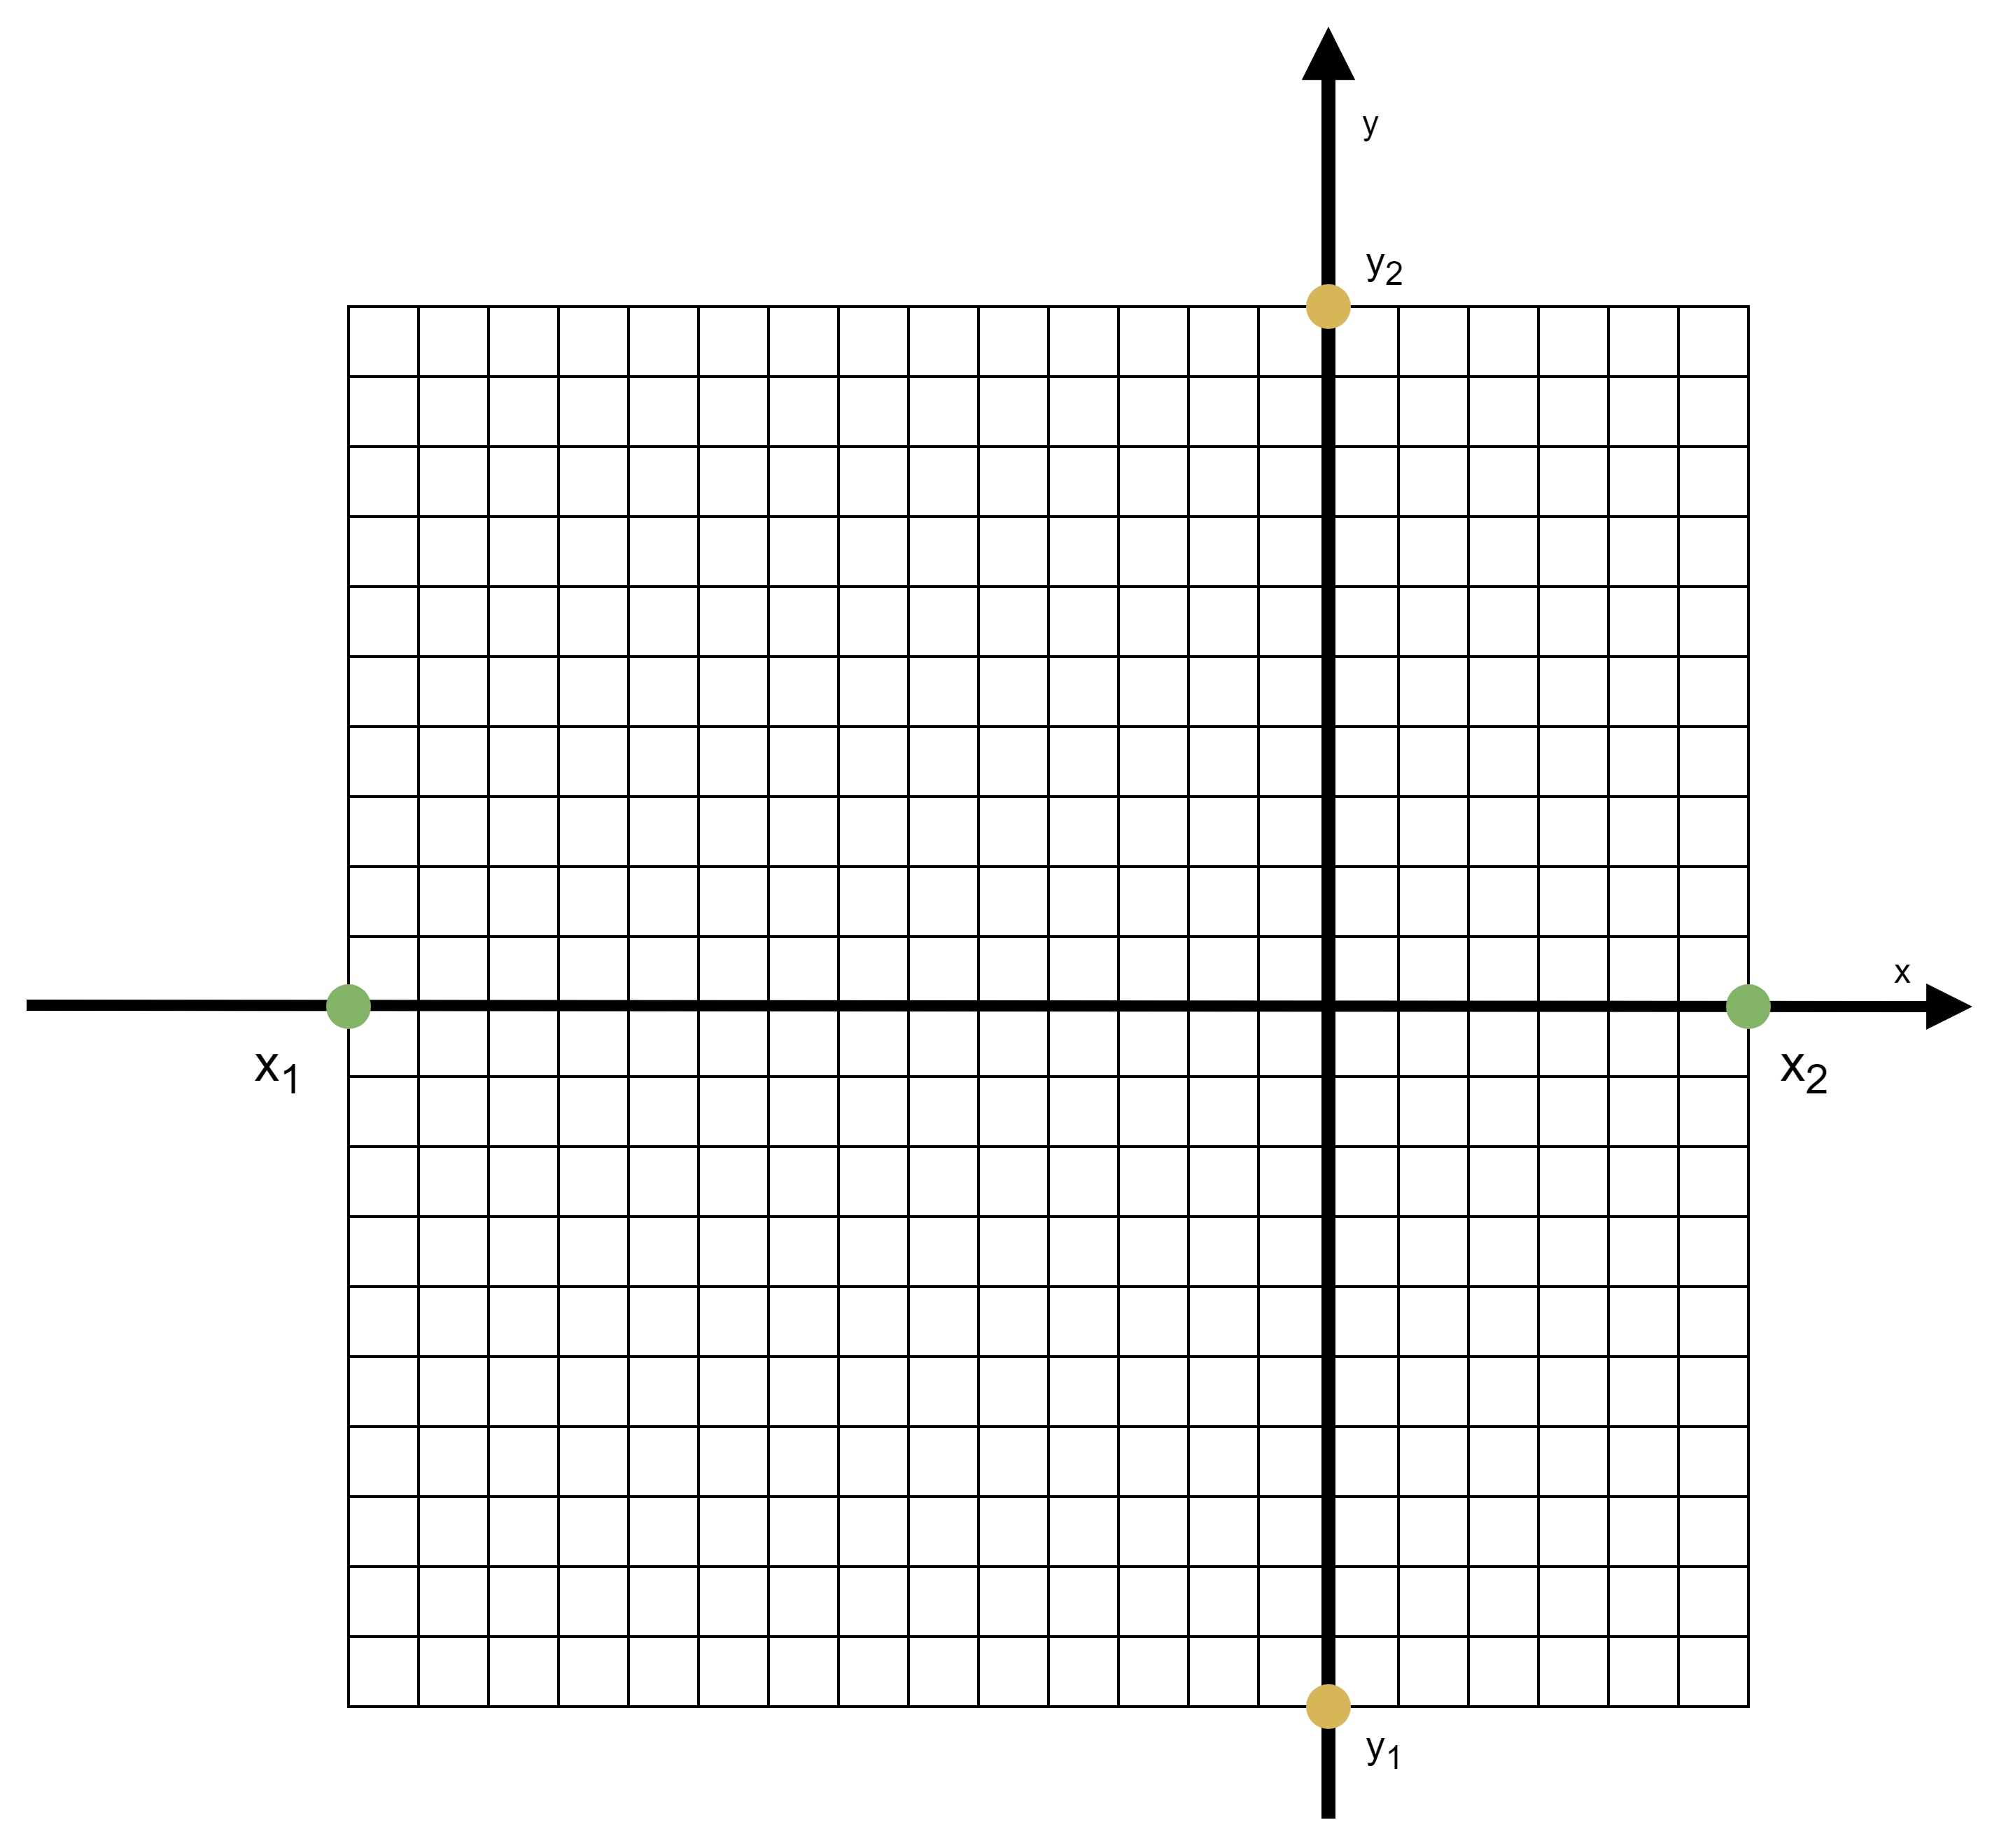
\includegraphics[width=0.6\linewidth]{image_to_coordinate.png}
    \caption{Piksellët në sistem kordinativ.}
    \label{fig:image_coordinate}
\end{figure}

\noindent \\ Duke zgjidhur për $x$ fitojmë
\[
\frac{i - 0}{w - 0} = \frac{x - x_1}{x_2 - x_1} \implies \frac{i}{w} = \frac{x - x_1}{x_2 - x_1} \implies x - x_1 = \frac{i}{w} (x_2 - x_1) \implies x = \frac{i}{w} (x_2 - x_1) + x_1
\]

\noindent \\ Në mënyrë krejtësisht analoge fitojmë

\[
y = \frac{j}{w} (y_2 - y_1) + y_1
\]

\noindent \\ Përfundimisht, pikselli $(i,j)$ pasqyrohet në pikën $(x,y)$ në sistemin kordinativ me anë të këtyre formulave:
\[
x = \frac{i}{w} (x_2 - x_1) + x_1
\]
\[
y = \frac{j}{h} (y_2 - y_1) + y_1
\]

\section{Ngjyrosja e Mandelbrot}

\noindent \\ Ngjyrosja e bashkësisë të Mandelbrot ka të bëjë me caktimin e ngjyrave të pikave në rrafshin kompleks bazuar se sa shpejtë vargu \(z_n\) tenton në infinit. Do të na duhej një numër \(t\) prej 0 në 1 për të reprezentuar këtë shpejtesi. Kjo vlerë pastaj konvertohet në sistemin e ngjyrave HSV e pastaj në RGB. 

\noindent \\ Ka shumë mënyra se si mund të llogaritet numri \(t\). Le të jetë \(n_\text{max}\) numri maksimal i iterimeve. Le të jetë  \(n\) numri i iterimit në të cilin \(z_n\) ose shpëton nga bashkësia e Mandelbrot  (\(n< n_\text{max}\)) ose mbetet mrenda bashkësisë dhe nuk shpëton (\(n=n_\text{max}\)). Mënyra më bazike e llogaritjes së numrit \(t\) është:

\[ t = \frac{n}{n_{\text{max}}} \]

\noindent Një menyre tjetër është duke shfrytëzuar formulën që njihet si normalized iteration count \cite{complex_colors}. Formula ipet:  
\[  s = n + 1 - \frac{\log(\log(|z_n|))}{\log(2)}\]

\noindent Vlera \(s\) normalizohet ndaj numrit maksimal të iterimeve: 
\[t = \frac{s}{n_{\text{max}}}\]
% \begin{align*}
%    \\
    
% \end{align*}

\noindent \\ Le të jetë treshja e ngjyrave në sistemin HSV $(H_{HSV}, S_{HSV}, V_{HSV})$, ku $H_{HSV}, S_{HSV}$, dhe $V_{HSV} \in [0,1]$. Vlera e nuancës në rastin tonë do të jetë $H = t$, e ngopjes $S_{HSV} = 1$, dhe e ndriçimit $V_{HSV} = 1$. Konvertimi i kësaj treshe në sistemin RGB bëhet sipas procesit të mëposhtëm \cite{hsv_rgb}.

\begin{align*}
H' &= (6 \cdot H_{HSV}) \mod 6  \\
c_1 &= \lfloor H' \rfloor, \quad c_2 = H' - c_1 \\
x &= (1 - S_{HSV}) \cdot v \\
y &= (1 - (S_{HSV} \cdot c_2)) \cdot V_{HSV} \\
z &= (1 - (S_{HSV} \cdot (1 - c_2))) \cdot V_{HSV}
\end{align*}

\noindent  Bazuar në  vlerën e  $c_1$, vlerat e normalizuara $R', G', B' \in [0,1]$ llogariten nga $v = V_{HSV}$, $x$, $y$, dhe $z$ si vijon:

\[
(R', G', B') = 
\begin{cases}
    (v, z, x) & \text{nëse } c_1 = 0 \\
    (y, v, x) & \text{nëse } c_1 = 1 \\
    (x, v, z) & \text{nëse } c_1 = 2 \\
    (x, y, v) & \text{nëse } c_1 = 3 \\
    (z, x, v) & \text{nëse } c_1 = 4 \\
    (v, x, y) & \text{nëse } c_1 = 5.
\end{cases} 
\]

\noindent \\  Përfundimisht bëhet shkallëzimi i RGB në numra të plotë në intervalin $[0, N - 1]$ (zakonisht $N = 256$).

\[
R = \min(\text{round}(N \cdot R'), N - 1),
\]
\[
G = \min(\text{round}(N \cdot G'), N - 1),
\]
\[
B = \min(\text{round}(N \cdot B'), N - 1). 
\]

\noindent Aplikimi i këtyre ngjyrave rezulton në imazhin \ref{fig:big_mandelbrot} dhe pasi që zmadhojmë në fraktal ngjyrat duken si në figurën \ref{mandelbrot_minis}.

 \begin{figure}[htbp]
\centering
\subfigure[]{
\includegraphics[width=83px,height=83px]{mandelbrot_3}}
\subfigure[]{
\includegraphics[width=83px,height=83px]{mandelbrot_4}}
\subfigure[]{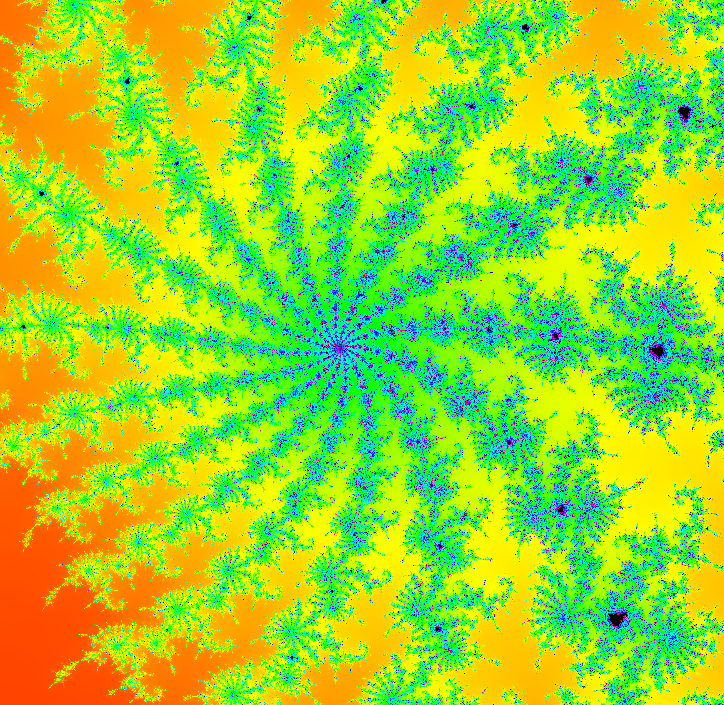
\includegraphics[width=83px,height=83px]{mandelbrot_5}}
\subfigure[]{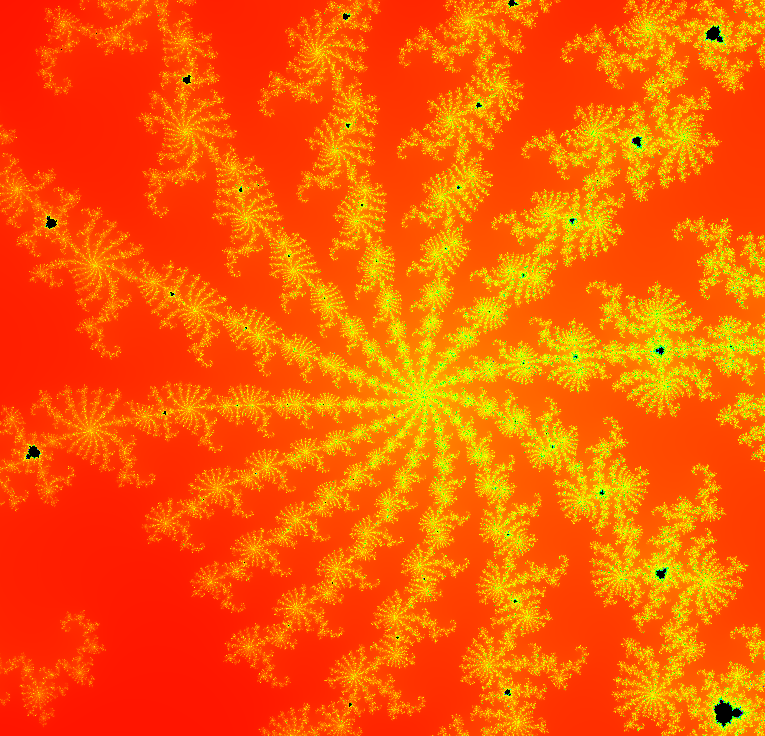
\includegraphics[width=83px,height=83px]{mandelbrot_6}}
\caption{Zmadhimet në bashkësinë Mandelbrot.}
\label{mandelbrot_minis}
\end{figure}


\newpage
\section{Kerneli}
Kerneli i mëposhtëm gjeneron një imazh të bashkësisë Mandelbrot. Secili thread i korrespondon një piksell të këtij imazhi. Fillimisht llogariten kordinatat komplekse të secilit piksell bazuar në indeksin e thredave. Pastaj fillon iterimi duke përdorur formulën e Mandelbrot për të caktuar nëse një piksell shpëton nga bashkësia mbrenda një numër të caktuar të iterimeve. Ngjyrat RGB caktohen bazuar në numrin e iterimit në të cilën \(z_n\) terminohet, dhe ngjyrat ruhen në vargun dalës për vizualizim. \\

\begin{lstlisting}
   __global__ void kernel(uchar4* ptr, double zoomfactor, double shiftX, double shiftY, int iterations, int width, int height) {

    int i = threadIdx.x + blockIdx.x * blockDim.x;
    int j = threadIdx.y + blockIdx.y * blockDim.y;
        
    int offset = i + j * blockDim.x * gridDim.x;
        
    double aspectRatio = (1.0 * width) / (1.0 * height);
    double startIntervalX = (-2) * zoomfactor * aspectRatio;
    double endIntervalX = 1 * zoomfactor * aspectRatio;
    double startIntervalY = 1.5 * zoomfactor;
    double endIntervalY = -1.5 * zoomfactor;
        
    //Each pixel represents a point in the Oxy coordinate system. These points are 
    double x = (endIntervalX - startIntervalX) * i / (width * 1.0) + startIntervalX + shiftX;
    double y = (endIntervalY - startIntervalY) * j / (height * 1.0) + startIntervalY + shiftY;
        
    double c_x = x;
    double c_y = y;
    double zX = 0, zY = 0, a = 0, b = 0;
    int max_iteration = iterations;
    int iteration;
    double squaredSums;
    for (iteration = 0; iteration < max_iteration; iteration++) {
        double zX_squared = zX * zX;
        double zY_squared = zY * zY;
        a = zX_squared - zY_squared + c_x;
        b = 2 * zX * zY + c_y;
        zX = a;
        zY = b;
        squaredSums = zX_squared + zY_squared;
        if (squaredSums > 4) {
            break;
        }
    }
    int R = 0, G = 0, B = 0;
    if (iteration < max_iteration) {
    setRGB(squaredSums, iteration, max_iteration, R, G, B);
    }
    ptr[offset].x = R;
    ptr[offset].y = G;
    ptr[offset].z = B;
    ptr[offset].w = 0;
} 
\end{lstlisting}

\section{Krahasimet}

\noindent Tabela \ref{tab:mandelbrot_table} krahason kohën e ekzekutimit në mikrosekonda për iterime të ndryshme të fraktalit ndërmjet versionit sekuencial dhe të versionit paralel në rezolucion 1920x1080.  Vizualizimi i këtyre rezultateve është bërë në figurën \ref{fig:mandelbrot_graph}.

\vspace{10pt} % Add some vertical space before the table

\begin{table}[h]
\centering
\resizebox{0.45\textwidth}{!}{%
\begin{tabular}{|l|l|l|}
\hline
Iterime & Sekuencial & CUDA \\ \hline
100 & 733630 & 9400 \\ \hline
130 & 843132 & 10436 \\ \hline
160 & 937728 & 11135 \\ \hline
190 & 1072441 & 11930 \\ \hline
210 & 1133325 & 12447 \\ \hline
255 & 1266945 & 15498 \\ \hline
445 & 1935680 & 14152 \\ \hline
610 & 2493841 & 16123 \\ \hline
775 & 3098080 & 19263 \\ \hline
1065 & 4057208 & 30757 \\ \hline
2300 & 8331929 & 63800 \\ \hline
\end{tabular}
}
\caption{Krahasimi i performancës.}
\label{tab:mandelbrot_table}
\end{table}


\begin{figure}[h]
\centering
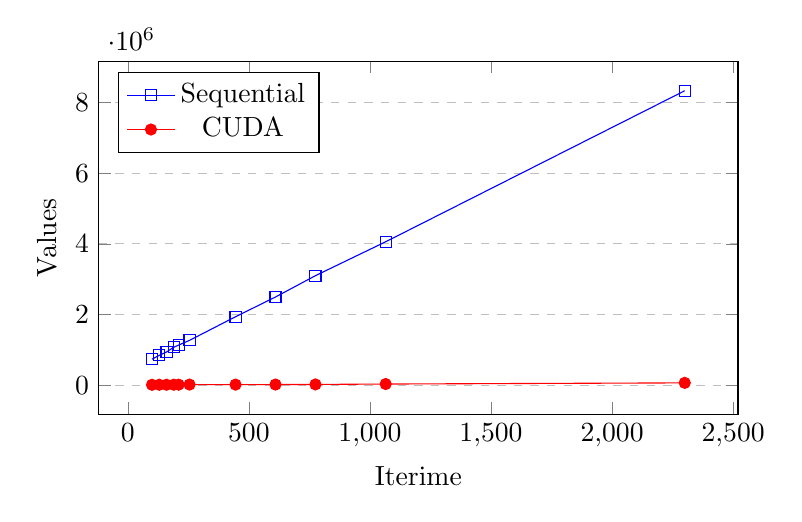
\begin{tikzpicture}
\begin{axis}[
    title={},
    xlabel={Iterime},
    ylabel={Values},
    legend pos=north west,
    ymajorgrids=true,
    grid style=dashed,
    width=0.8\textwidth,  % Adjust width as needed
    height=0.5\textwidth, % Adjust height as needed
]
\addplot[
    color=blue,
    mark=square,
    ]
    coordinates {
    (100,733630)(130,843132)(160,937728)(190,1072441)(210,1133325)(255,1266945)(445,1935680)(610,2493841)(775,3098080)(1065,4057208)(2300,8331929)
    };
\addplot[
    color=red,
    mark=*,
    ]
    coordinates {
    (100,9400)(130,10436)(160,11135)(190,11930)(210,12447)(255,15498)(445,14152)(610,16123)(775,19263)(1065,30757)(2300,63800)
    };
\legend{Sequential, CUDA}
\end{axis}
\end{tikzpicture}
\caption{Grafiku i krahasimit të performancës.}
\label{fig:mandelbrot_graph}
\end{figure}



\newpage

\begin{figure}[]
    \centering
    \makebox[\textwidth]{
\includegraphics[width=1.6\linewidth]{mandelbrot_2}}
    \caption{Mandelbrot Set i gjeneruar me CUDA.}
    \label{fig:big_mandelbrot}
\end{figure}


